\documentclass[pdftex,12pt,letter]{article}
\usepackage{fancyhdr}
\usepackage{enumerate}
\usepackage{tabularx}
\usepackage{graphicx}
\usepackage{array}
\usepackage[justification=justified,singlelinecheck=false]{caption}
\pagestyle{fancy}
\makeatletter
  \renewcommand\@seccntformat[1]{\csname the#1\endcsname.\quad}
\makeatother

\newcolumntype {Y}{ >{\raggedright \arraybackslash }X}
\newcommand{\HRule}{\rule{\linewidth}{0.5mm}}
\captionsetup{labelformat=empty}

\begin{document}

\begin{titlepage}
\begin{flushright}
\HRule \\[0.4cm]
{ \bfseries
{\huge Software Requirements Specification\\[1cm]}
{\Large for\\[1cm]}
{\huge CWRUtility\large{\footnote[1]{Working title}}\\[4cm]}
{\large Prepared by\\Jason Kuster, Stuart Long, and William Ordivay\\[1cm]
Version 1.0\\[1cm]
KOALAA Development\\[1cm]
October 1, 2012}}
\end{flushright}
\end{titlepage}
\tableofcontents{}
\vspace{5cm}
\begin{table}[h]
\caption*{\bfseries Revision History}
\begin{tabularx}{\textwidth }[t]{|l|Y|Y|Y|}
\hline
\bfseries Name & \bfseries Date & \bfseries Reasons for Change & \bfseries Version \\ \hline
Kuster, Long, Ordiway & 9/22/2012 & Initial Draft & 1.0 draft 1\\ \hline
\end{tabularx}
\end{table}
\newpage
\section{Introduction}
\subsection{Purpose}
This Software Requirements Specification describes the software functional and nonfunctional requirements for release 1.0 of CWRUtility. This specification document is intended for the solu use of the members of the project team that will implement and verify the correction functioning of the system. Unless otherwise specified, all requirements documented here are high priority and committed for release 1.0. 

\subsection{Business Objectives and Success Criteria}
\begin{enumerate}[BO-1:]
\item Reduce difficulty experienced by new students due to unfamiliar CWRU environment.
\item Increase general efficiency of CWRU students and faculty by facilitating their uses of certain CWRU resources.
\item Centralize access to most commonly used CWRU resources.
\end{enumerate}

\begin{enumerate}[SC-1:]
\item 50\% of all Windows phone users in the Case community actively use the application.
\item Application received at least 10 positive reviews on the Windows Marketplace.
\item 3 months after release, more positive reviews then negative reviews.
\item Recognition of application in university literature (such as \emph{The Case Daily})
\end{enumerate}


\subsection{Business Risks}
\begin{enumerate}[BR-1:]
\item Application fails certification for the Windows Phone Store.
\item Windows Phone is a currently less utilized application platform than its competitors, increasing the risk that fewer students will use the application.
\end{enumerate}

\section{Vision of the Solution}
\subsection{Vision Statement}
For students who currently struggle with knowing where their classes are, getting to classes on time, or using the myriad of other resources CWRU provides to its students, CWRUtility is an app which will solve these problems. It is an elegantly designed mobile application which will provide useful information and centralize the services students use most.
\subsection{Major Features}
\begin{enumerate}[FE-1:]
\item Integrates with the Student Information System to schedule students' courses.
\item Provide map of CWRU campus with detailed information on students' course locations.
\item Integrates with NextBus, Inc. to provide a schedule for the "greenie" system.
\item Displays hours, locations, and other  such information for Case services
\item Displays menus for both major dining halls.
\item Lists phone numbers of important Case resources, such as campus security.
\item Integrates with \emph{The Case Daily} to display daily news.
\item Integrates with the e-Suds system to provide laundry information.
\item Provides the current 5-year academic calendar.
\item Displays the RSS feed of the \emph{Case Western Observer}.
\end{enumerate} 
\subsection{Assumptions and Dependencies}
\begin{enumerate}[{A}S-1:]
\item Mobile device is equipped with an internet connection.
\end{enumerate}
\begin{enumerate}[DE-1:]
\item This application depends on the continuing functionality of the described services.
\end{enumerate}
\section{Scope and Limitations}
\subsection{Scope of Initial and Subsequent Releases}
\begin{table}[h]
\begin{tabularx}{\textwidth }[t]{|l|Y|Y|Y|}
\hline
\bfseries Feature & \bfseries\hspace{1cm}Release 1 & \bfseries\hspace{1cm}Release 2 & \bfseries\hspace{1cm}Release 3 \\ \hline
FE-1 & Fully implemented & ~ & ~ \\ \hline
FE-2 & Basic map & Integrated with course schedule & Provides directions \\ \hline
FE-3 & Basic functionality with NextBus & Full integration with NextBus (if needed) & Integration with Map \\ \hline
FE-4 & Fully implemented & ~ & ~ \\ \hline
FE-5 & Not implemented & Fully implemented & ~ \\ \hline
FE-6 & Fully implemented & ~ & ~ \\ \hline
FE-7 & Not implemented & Fully implemented & ~ \\ \hline
FE-8 & Not implemented & Basic information displays & Integrates with phone's notification system \\ \hline
FE-9 & Table of events & ~ & Integrated with course schedule \\ \hline
FE-10 & Not implemented & Fully implemented & ~ \\
\hline
\end{tabularx}
\end{table}
\subsection{Limitations and Exclusions}
\begin{enumerate}[L{I}-1:]
\item Requires functioning internet connection.
\item Dependency on external services.
\end{enumerate}
\begin{enumerate}[EX-1:]
\item Available only for Windows Phone 7 / Windows Phone 8 mobile devices.
\end{enumerate}
\section{Business Context}
\subsection{User Profile}
\begin{table}[h]
\begin{tabularx}{\textwidth}[t]{|Y|Y|Y|Y|}
\hline
\bfseries User & \bfseries Value & \bfseries Interests & \bfseries Constraints\\ \hline
CWRU community members & More efficient and centralized use of CWRU services and resources & Ease of use; reliability; simplicity & Required to have a Windows Phone 7/8 with internet access \\ \hline
CWRU service providers & increased discoverability and utilization of their services & Appropriate representation of services in software & Potential for communication with CWRUtility to malfunction after service updates \\ \hline
\end{tabularx}
\end{table}

\lfoot{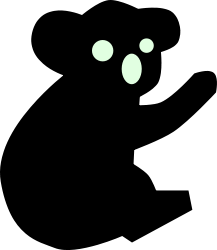
\includegraphics[height=1cm]{DarkKoala.png}}
\end{document}